\section{POMDP-based Problem Formulation}
\label{sec:formulation}
%----------------------------------------------------------------------------------------%
In this section, we formulate the optimization of job dispatching problem of all APs as a Markov decision process (MDP).
Since each AP updates the job dispatching action according to OSI instead of GSI, the MDP problem is a partially observable MDP (POMDP).
Firstly, we give the definitions of \emph{dispatching policy} and \emph{cost function}, together with the \emph{system state} (i.e., the GSI) defined previously, to complete the MDP problem formulation.
% Specifically, the individual dispatching policy of one AP, the system dispatching policy, and the cost function are first defined below.

\begin{definition}[Dispatching Policy]
    The individual dispatching policy of the $k$-th AP, denoted as $\Omega_{k}$ ($\forall k \in\apSet$), maps from its OSI $\Stat_{k}$ and its \brlatency~$\mathcal{D}_{k}$ to the dispatching action for each job type, i.e.,
    \begin{align}
        \Omega_{k} \Paren{ \Stat_{k}(t), \mathcal{D}_{k}(t) }
        &\define \mathcal{A}_{k}(t+1)
        \nonumber\\
        &= \Brace{
            \omega_{k,j}(t+1) \Big| \forall j\in\jSpace
        }.
        \label{def:action}
    \end{align}

    The aggregation of individual policy of all APs is referred to as the system dispatching policy $\Policy$.
    Thus,
    {\small
    \begin{align}
        \Policy\Paren{ \Stat(t), \Delay(t) } \define \Brace{
            \Omega_{1}(\Stat_{1}(t), \mathcal{D}_{1}(t)), \dots, \Omega_{K}(\Stat_{K}(t),\mathcal{D}_{K}(t))
        },
    \end{align}
    }
    where $\Delay(t) \define \set{ \mathcal{D}_{1}(t), \dots, \mathcal{D}_{K}(t) }$.
\end{definition}

\revision{
    In this paper, the average job response time and packet drop rate are considered as the system cost.
    The job response time counts the number of broadcast intervals from job arrival to the accomplishment of computation, which includes the uploading time from the AP to the edge server, the waiting time in the processing queue and the job processing time on the edge server.
    According to the Little's law \cite{Little1961}, the average response time per job is proportional to the number of jobs in the system, given the job arrival rates at all the APs.
    % According to the Little's law \cite{Little1961}, the average response time per job, counting the number of broadcast intervals from job arrival to the accomplishment of computation, is proportional to the number of jobs in the system, given the job arrival rates at all the APs. %broadcast intervals
}%
Hence, we define the cost function per broadcast interval as follows, {given the information contained in periodic broadcast.}

\begin{definition}[Cost Function per Broadcast Interval]
    The cost function of the $t$-th broadcast interval with GSI $\Stat(t)$ is defined as
    {\small
    \begin{align}
        g\Paren{\Stat(t)} \define
            \sum_{m\in\esSet,j\in\jSpace}
            \Brace{&
                \sum_{k\in\apSet} \Inorm{\vec{R}^{(k)}_{m,j}(t,0)} + Q_{m,j}(t,0)
                \nonumber\\
                &~~~~~+ \beta \cdot I[Q_{m,j}(t,0)=L_{max}]
            },
    \end{align}
    }%
    where $\Inorm{\vec{x}}$ denotes the $L^1$-norm of the vector $\vec{x}$, $\sum_{k\in\apSet} \Inorm{\vec{R}^{(k)}_{m,j}(t,0)}$ measures the number of type-$j$ jobs being uploaded from the $k$-th AP to the $m$-th edge server, $Q_{m,j}(t,0)$ measures the number of type-$j$ jobs on the $m$-th edge server, and $\beta$ is the weight of overflow penalty.
    \deny{
        The cost function per broadcast interval could be taken as a uniform sampling of cost function per time slot.
    }
\end{definition}

Since the job dispatching in one broadcast interval will affect the GSI of the following broadcast intervals, we should consider the joint minimization of the costs of all the broadcast intervals.
Specifically, we consider the following discounted sum of the costs of all the broadcast intervals as the system objective.
{\small
\begin{align}
    &\bar{G}(\Stat(1), \Policy) \define
    \lim_{T \to \infty} \mathbb{E}^{\Policy}_{\set{\Stat(t)|\forall t}, \Delay}
    \Bracket{
        \sum_{t=1}^{T} \gamma^{t-1} g\Paren{\Stat(t)} \Big| \Stat(1)
    },
\end{align}
}%
where $\mathbb{E}^{\Policy}_{\set{\Stat(t)|\forall t}}[\cdot]$ denotes the expectation with respect to all possible system states in the future given scheduling policy $\Policy$, and $\gamma \in (0,1)$ is the discount factor.
Hence, the optimization of job dispatching policy can be formulated as the following minimization problem.
\begin{align}
    \textbf{P1:}~
    \min_{\Policy} \bar{G}(\Stat(1), \Policy).
\end{align}

If the GSI $\Stat(t)$ and \brlatency~$\Delay(t)$ are known to all the APs, the MDP in problem P1 can be solved via the following Bellman's equations as in \cite{sutton1998}.
\begin{align}
    &V\Paren{\Stat(t)} =g\Paren{\Stat(t)}
        + \gamma\mathbb{E}_{\Delay}\bigg\{
            \min_{\Policy(\Stat(t),\Delay(t))}
            \nonumber\\
            &\sum_{\Stat(t+1)} \Pr \Big\{ 
                \Stat(t+1) \Big| \Stat(t), \Policy(\Stat(t), \Delay(t)) \Big\} \cdot V\Big(\Stat(t+1)\Big)
            \bigg\},
    \label{eqn:sp_0}
\end{align}
where the value function $V(\Stat(t))$ of the optimal policy $\Policy^{*}$ (if GSI and \brlatency~are known to all the APs) is defined as follows.
\begin{align}
    &V\Paren{\Stat(t)} \define
    \lim_{T\to\infty} 
    \mathbb{E}^{\Policy^*}_{\set{\Stat(t)|\forall t}, \Delay} \Bracket{
        \sum_{t=1}^{T} \gamma^{t-1} g\Big( \Stat(t) \Big) \Big| \Stat(1)
    }.
    \label{eqn:val_f}
\end{align}
Moreover, the optimal dispatching policy $\Omega^{*}$ can be obtained by solving the right-hand-side (RHS) of the above Bellman's equations (\ref{eqn:sp_0}).

However, it is infeasible to solve the above Bellman's equations {and achieve the performance of $\Policy^*$ in our considered distributed dispatching scenario.}
This is because each AP (say the $k$-th AP) only has the knowledge of its own OSI $\Stat_{k}(t)$ and local \brlatency~$\mathcal{D}_{k}(t)$, but the optimal solution (dispatching actions of all APs) for the RHS of equation (\ref{eqn:sp_0}) depends on the GSI and the knowledge of global \brlatency.
Thus, problem P1 is actually a POMDP\revision{, which is further demonstrated by a toy example below.}
\revision{
    \begin{figure}[htp!]
        \centering
        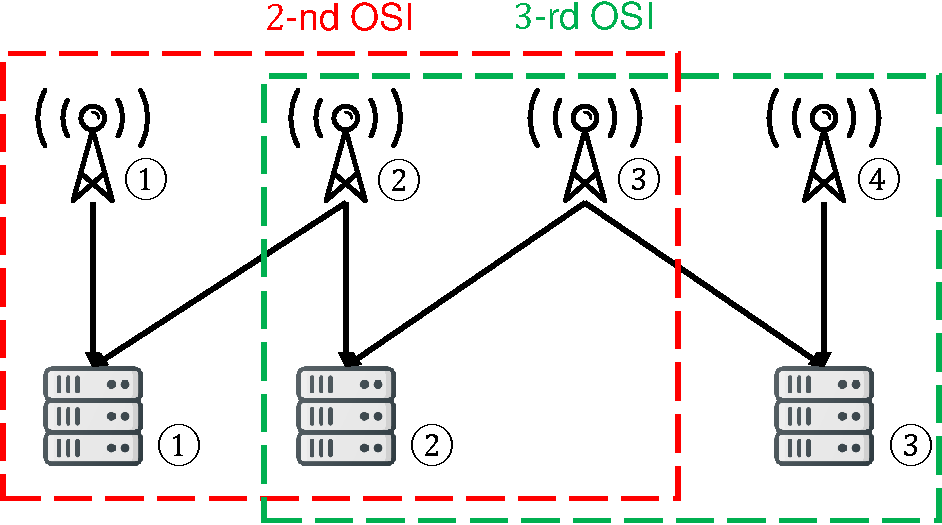
\includegraphics[width=0.45\textwidth]{images/osi-example.pdf}
        \caption{An example of system model, where the edge servers $1,2,3$ are collocated with the APs $1,2,4$, respectively.}
        \label{fig:osi_example}
    \end{figure}

    \begin{example}
        {%
            As illustrated in Fig.\ref{fig:osi_example}, there are four APs and three edge servers collocated with the APs, in the edge computing system, where the solid directed lines show all the possible job dispatching paths for the APs.
            For the $2$-nd AP, its OSI includes the state information of the APs indexed with $1,3$ and the edge servers indexed with $1,2$.
            The state information of the $3$-rd edge server is out of its scope.
            Moreover, the OSI of the $3$-rd AP (namely, the $3$-rd OSI) includes the state information of the APs indexed with $2,4$ and the edge servers indexed with $2,3$.
        }%
        Note that the prediction of future state distribution is essential for solving the RHS of equation (\ref{eqn:sp_0}).
        {%
            Without GSI, it is impossible to predict the future dispatching decisions of the $3$-rd AP from the perspective of the $2$-nd AP, since they observe different OSIs.
            It is thereby impossible for the $2$-nd AP to predict the future state distributions of the $2$-nd edge server, lack of the dispatching decisions of the $3$-rd AP.
            As a result, the evaluation of optimal value function of equation (\ref{eqn:val_f}) is infeasible at both $2$-nd and $3$-rd APs, and the distributed policy optimization for them is a POMDP.
        }
    \end{example}
}%

The general solution of POMDP is of huge complexity {as all the historical system states should be traced back in the current system state} \cite{IJCAI03-NairR,IJCAI99-BoutilierC}.
In this paper, we shall propose a novel low-complexity solution framework based on an analytical approximation of the value function $V(\cdot)$ and alternative actions update, where distributed job dispatching via the Bellman's equations becomes feasible
(the minimization at the RHS of equation (\ref{eqn:sp_0}) is solvable with the approximate value function)
even with OSI and local \brlatency.
%----------------------------------------------------------------------------------------%
